\documentclass[12pt,letterpaper]{article}

\usepackage[utf8]{inputenc}
\usepackage[spanish]{babel}
\usepackage{graphicx}
\usepackage[hidelinks]{hyperref}
\usepackage{hyperref}
\usepackage[left=2cm,right=2cm,top=2.5cm,bottom=2cm]{geometry}
\usepackage{graphicx}
\usepackage{float}
\usepackage{amsmath}
\usepackage{stackrel} 
\usepackage{multicol}
\usepackage{multirow}
\usepackage{fancyhdr}
\usepackage[usenames,dvipsnames,svgnames,table]{xcolor}
\usepackage[document]{ragged2e}
\usepackage{enumerate}

\usepackage{helvet}

\renewcommand{\labelitemi}{$-$}
\renewcommand{\labelitemii}{$\cdot$}
\newcommand\tab[1][1cm]{\hspace*{#1}}

\renewcommand{\familydefault}{\sfdefault}

\definecolor{azul}{RGB}{0,0,255}

\pagestyle{fancy}
\lhead{\begin{picture}(0,0) \put(0,0){
\includegraphics[width=10mm]{./img/logo}} \end{picture}}
\chead{\hspace{1cm}\vspace{0.2cm}Laboratorio 04 - Power BI dashboards adicionales}
\rhead{}

\begin{document}
    \begin{titlepage}
        \begin{center}
            \begin{figure}[htb]
                \begin{center}
                    
\includegraphics[width=3.5cm]{./img/logo}
                \end{center}
            \end{figure}
            \vspace*{0.15in}
            \begin{Large}
                \textbf{UNIVERSIDAD PRIVADA DE TACNA}\\
            \end{Large}
            \vspace*{0.15in}
            \begin{Large}
                \textbf{FACULTAD DE INGENIERÍA} \\
            \end{Large}
            \vspace*{0.1in}
            \begin{Large}
                \textbf{Escuela Profesional de Ingeniería de Sistemas} \\
            \end{Large}
            \vspace*{0.3in}
            \begin{Large}
                \textbf{Laboratorio 04}\\
                \textbf{``Power BI dashboards adicionales"}\\
            \end{Large}
            \vspace*{0.2in}
            \begin{Large}
                \textbf{CURSO:} \\
            \end{Large}
            \vspace*{0.1in}
            \begin{large}
                Inteligencia de Negocios\\
            \end{large}
            \vspace*{0.2in}
            \begin{Large}
                \textbf{DOCENTE:} \\
            \end{Large}
            \vspace*{0.1in}
            \begin{large}
                Mag. Patrick Jose Cuadros Quiroga\\
            \end{large}
            \vspace*{0.3in}
            \begin{large}
                \textbf{ALUMNO:} \\
                \begin{flushleft}
                    Lipa Calabilla, Abraham  		\hfill	(2019064039) \\
                \end{flushleft}
            \end{large}
            \vspace*{1.3in}
            \begin{large}
                Tacna - Perú\\
            \end{large}
            \vspace*{0.1in}
            \begin{large}
                2022\\
            \end{large}
        \end{center}
    \end{titlepage}
    \include{Secciones/articulo}
    \newpage
    \tableofcontents
    \justify
    \newpage
    \begin{LARGE}
        \begin{center}
            \textbf{POWER BI DASHBOARDS ADICIONALES} \\
        \end{center}
    \end{LARGE}
    
    \section{OBJETIVOS}
    \begin{itemize}
        \item Crear dashboards usando la herramienta Power BI.
    \end{itemize}
    
    \section{REQUERIMIENTOS}
    \begin{itemize}
        \item Conocimientos\\
        Para el desarrollo de esta práctica se requerirá de los siguientes conocimientos básicos:
        \begin{itemize} 
            \item Conocimientos básicos de administración de base de datos Microsoft SQL Server.
            \item Conocimientos básicos de SQL.
        \end{itemize}
        \item Hardware
        \begin{itemize}
            \item CPU SLAT-capable feature.
            \item Al menos 4GB de RAM.
        \end{itemize}
        \item Software\\
        Así mismo se necesitan los siguientes aplicativos
        \begin{itemize}
            \item Microsoft SQL Server 2017 o superior.
            \item Base de datos AdventureWorksLT2017 o superior.
            \item Tener los archivos de recursos del laboratorio.
            \item Power BI Desktop.
            \item Tener una cuenta Microsoft registrada en el Portal de Power Bi.
        \end{itemize}
    \end{itemize}
    
    \section{CONSIDERACIONES INICIALES}
    Microsoft Power BI es un conjunto de aplicaciones para el análisis empresarial, que permite unificar diferentes fuentes de datos, configura y analiza datos que son presentados de manera sencilla en tablas e informes, que pueden ser consultados de una manera muy fácil y atractiva en tiempo real por usuarios e integrantes de una misma empresa u organización.
    
    \newpage
    \section{DESARROLLO}
    \begin{enumerate}[\tab 1.]
        \item Para esta guía utilizaremos el cubo creado en la guía anterior. Inicie Power BI Desktop, busque y seleccione la opción Get Data.
        \begin{center}
            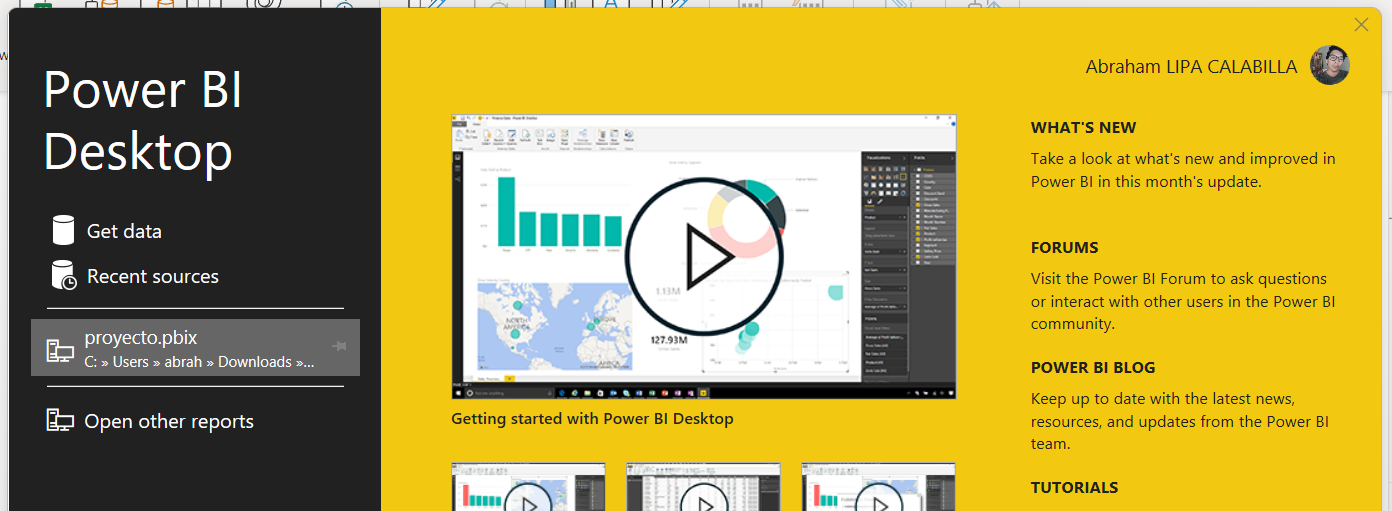
\includegraphics[width=13cm]{./img/img1.png}
        \end{center}
        \item Dentro de los resources seleccionaremos SQL Server database.
        \begin{center}
            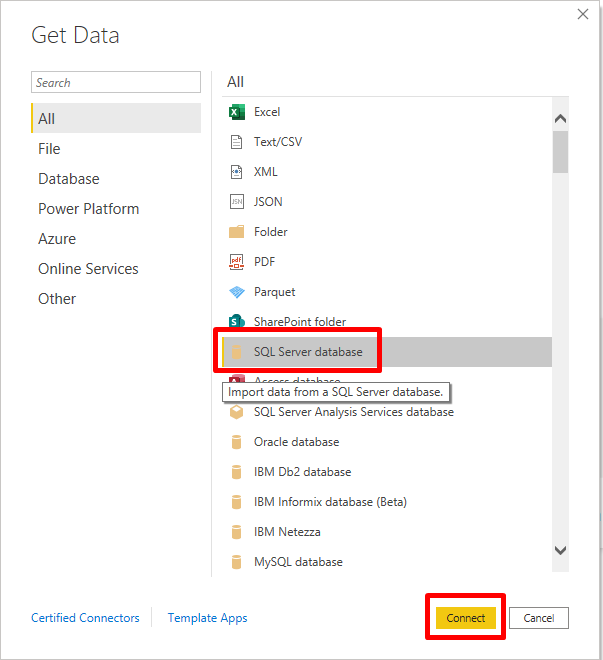
\includegraphics[width=7cm]{./img/img2.png}
        \end{center}
        \item Utilice el nombre de host o localhost para conectarse.
        \begin{itemize}
            \item Vamos a seleccionar Adventure Works DW2017.
            \begin{center}
                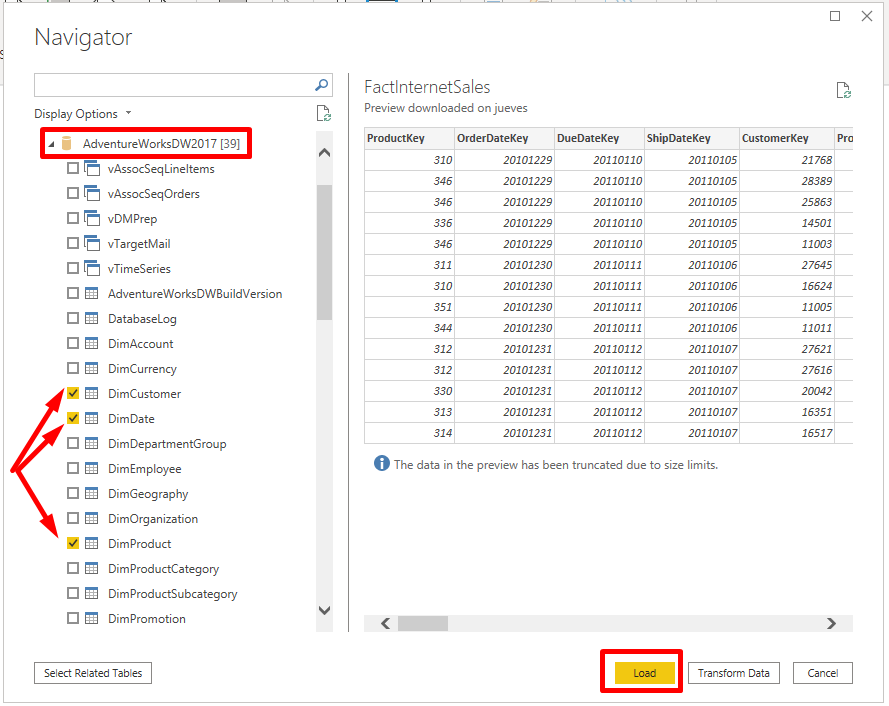
\includegraphics[width=13cm]{./img/img3.1.png}
            \end{center}
        \end{itemize}
        \item Una vez conectado tendremos en nuestro lado dos toolbox, uno denominado VISUALIZATONS y otro denominado FIELDS.
        \begin{itemize}
            \item En FIELDS debe mostrar la Fact Table de Internet Sales y las dimensiones asociadas según las guías previas de cubos.
            \begin{center}
                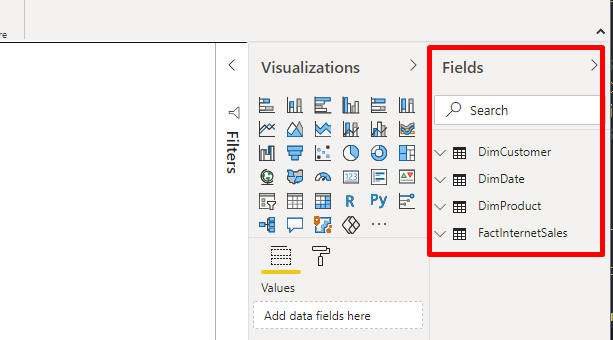
\includegraphics[width=8cm]{./img/img4.1.png}
            \end{center}
        \end{itemize}
        \item Vamos a crear nuestro primer reporte. Seleccionaremos una gráfica de barras, en segundo lugar Sales Amount, Calendar Year y English Product Name. (Debe hacerlo en ese orden).
        \begin{center}
            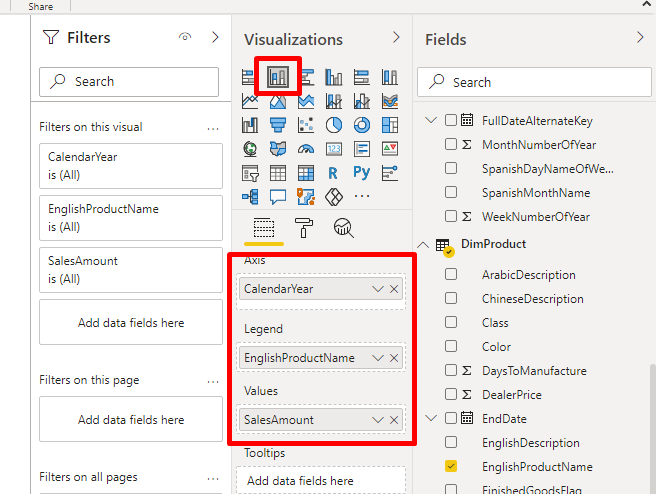
\includegraphics[width=8cm]{./img/img5.png}
        \end{center}
        \item La gráfica resultante es la siguiente:
        \begin{center}
            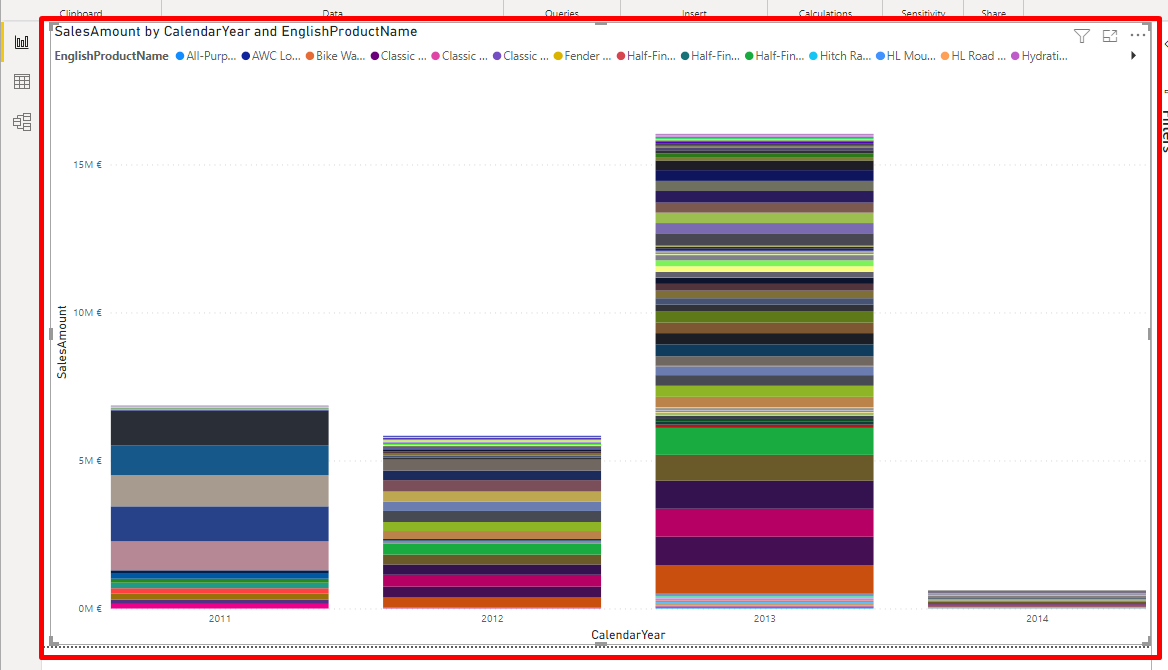
\includegraphics[width=13cm]{./img/img6.png}
        \end{center}
        \item Elimine la gráfica anterior y procederá a seleccionar gráfica de barras, en segundo lugar Sales Amount, English Product Name y Calendar Year. (Debe hacerlo en ese orden).
        \begin{center}
            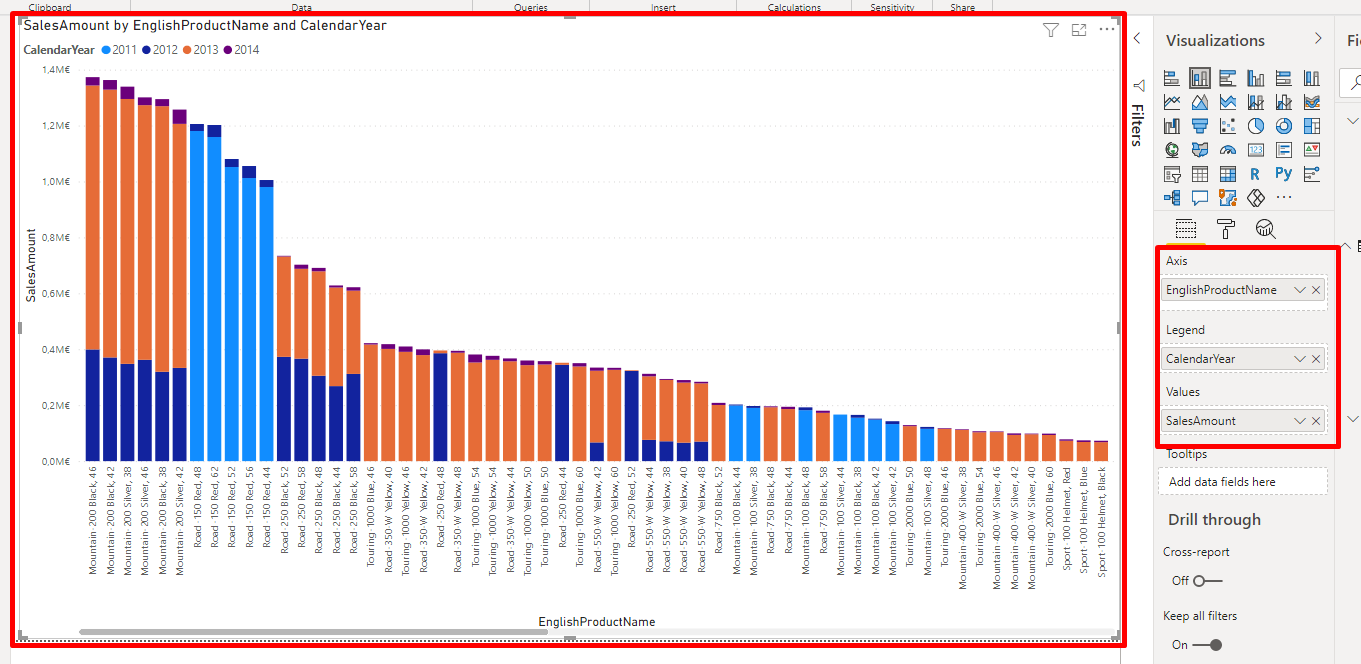
\includegraphics[width=13cm]{./img/img7.png}
        \end{center}
        La gráfica cambiará, lo que indica que el orden de agregado es importante para las visualizaciones, aún habiendo seleccionado los mismos datos.          
        \item Cree un nuevo reporte.
        \begin{center}
            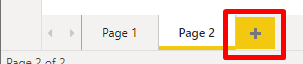
\includegraphics[width=5cm]{./img/img8.png}
        \end{center}
        \begin{itemize}
            \item Podemos crear un dashboard con gráficos simultáneos. Arrastre dos gráficas y seleccione una de ella para establecer las propiedades.
            \begin{center}
                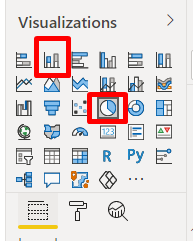
\includegraphics[width=5cm]{./img/img8.1.png}
            \end{center}
            \begin{center}
                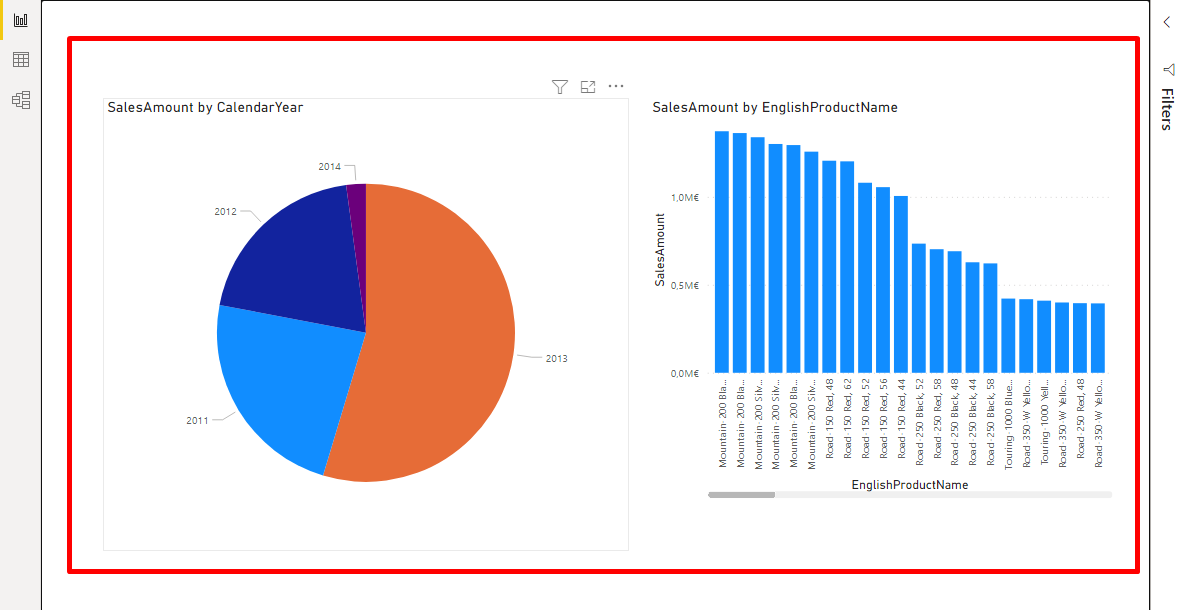
\includegraphics[width=13cm]{./img/img8.2.png}
            \end{center}
        \end{itemize}
        \item Seleccione una de los valores de la gráfica de la izquierda para ver el comportamiento:
        \begin{center}
            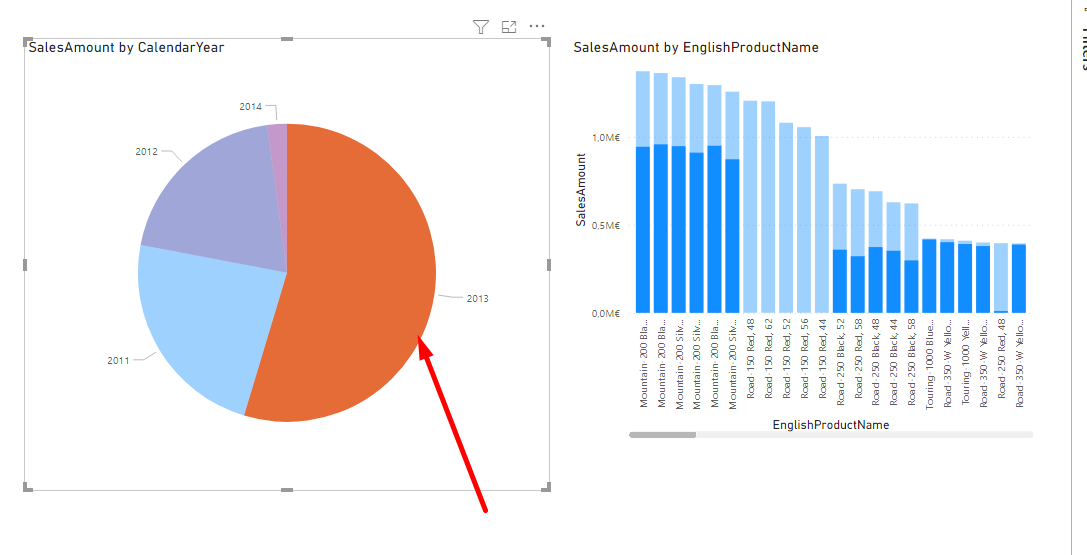
\includegraphics[width=13cm]{./img/img9.png}
        \end{center}
        \item Ahora crearemos un mapa que muestre la proporción de ventas por zona geográfica. Arrastre un Mapa y una tabla.
        \begin{center}
            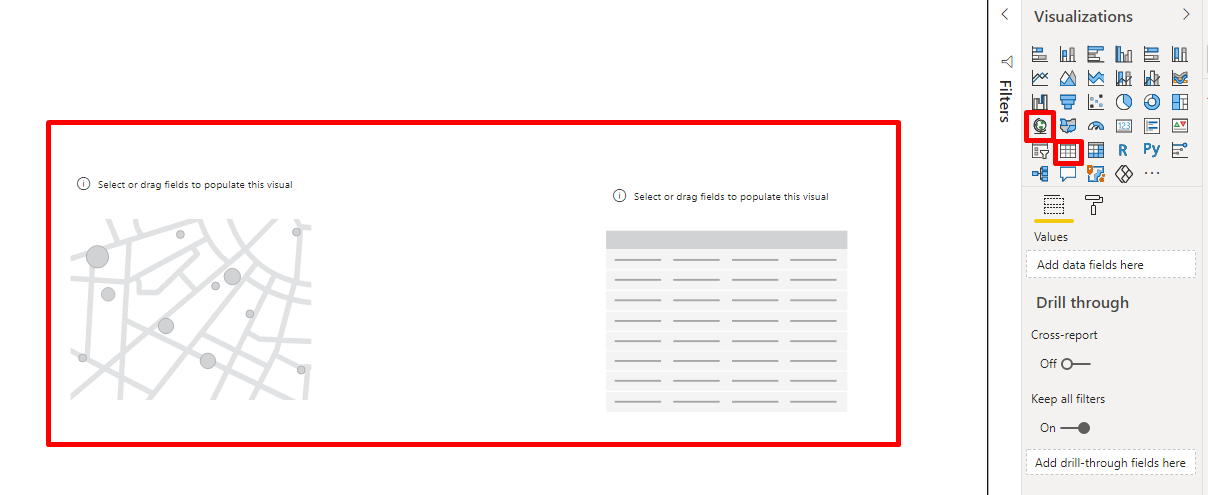
\includegraphics[width=13cm]{./img/img10.png}
        \end{center}
        \begin{itemize}
            \item Para este reporte se necesitara agregar una tabla nueva para sacar los datos, la cual es \textbf{DimGeography} y se usara el campo \textbf{EnlgishCountryRegionName}. 
            \begin{center}
                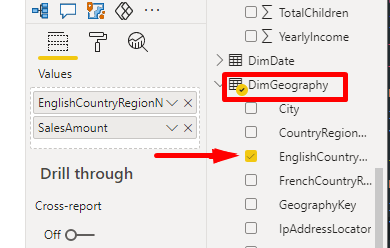
\includegraphics[width=8cm]{./img/img10.1.png}
            \end{center}
            \item El grafico se vera de la siguiente manera.
            \begin{center}
                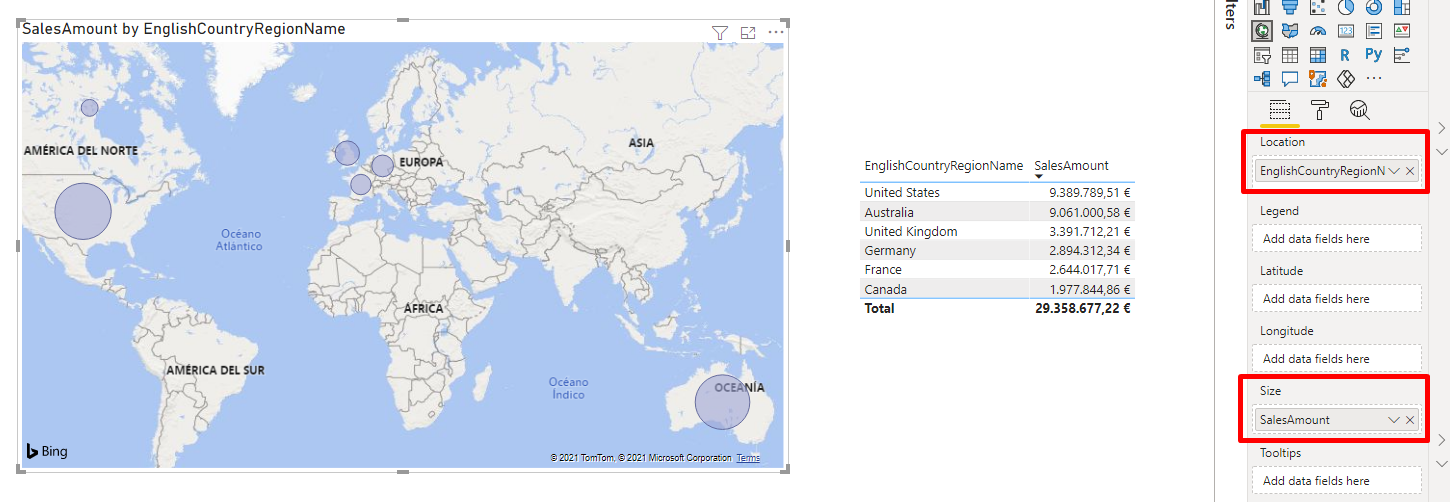
\includegraphics[width=13cm]{./img/img10.2.png}
            \end{center}
        \end{itemize}
        \item Ahora generaremos una gráfica de área.
        \begin{itemize}
            \item En primer lugar seleccione una nueva página y agregue una gráfica de área.
            \begin{center}
                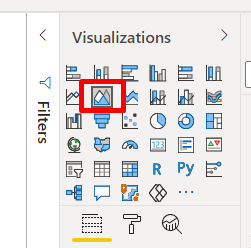
\includegraphics[width=5cm]{./img/img11.1.png}
            \end{center}
            \item Luego seleccione las medidas que se van a mostrar en el gráfico:
            \begin{center}
                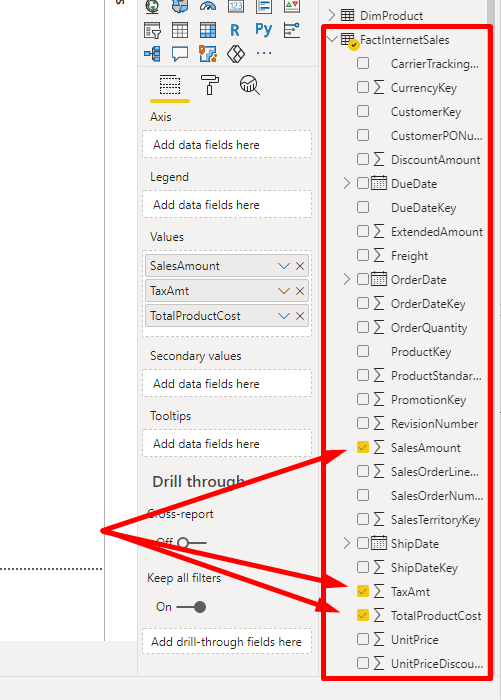
\includegraphics[width=8cm]{./img/img11.2.png}
            \end{center}
            \item Ordene el resultado por año de manera ascendente.
            \begin{center}
                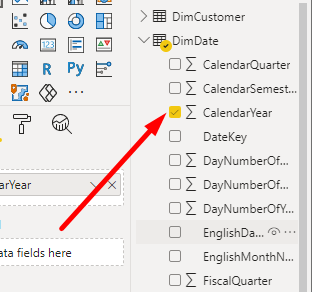
\includegraphics[width=5cm]{./img/img11.3.png}
            \end{center}
        \end{itemize}
        \item Agregaremos una gráfica de líneas. Vamos a seleccionar desde la tabla de hecho a Sales Amount.
        \item A continuación agregaremos Calendar Year desde Order Date y luego English Country Region Name. Debe realizarse en este orden o el resultado será diferente.
        \begin{center}
            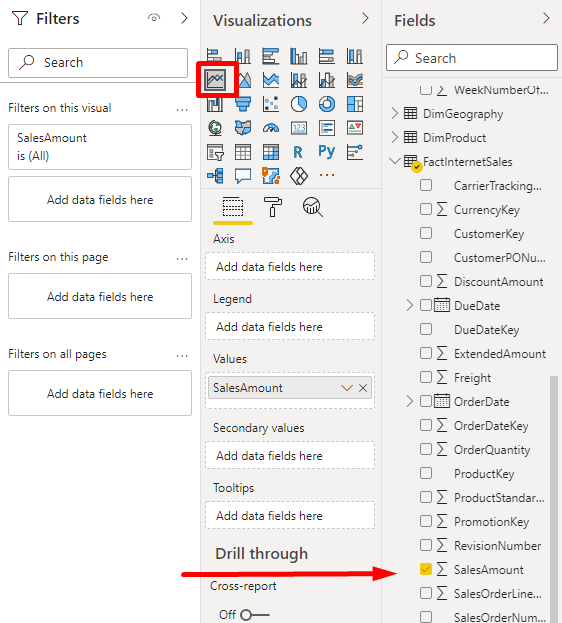
\includegraphics[width=13cm]{./img/img12.1.png}
        \end{center}
        \begin{itemize}
            \item A continuación agregaremos Calendar Year desde Order Date y luego English Country Region Name. Debe realizarse en este orden o el resultado será diferente.
            \begin{center}
                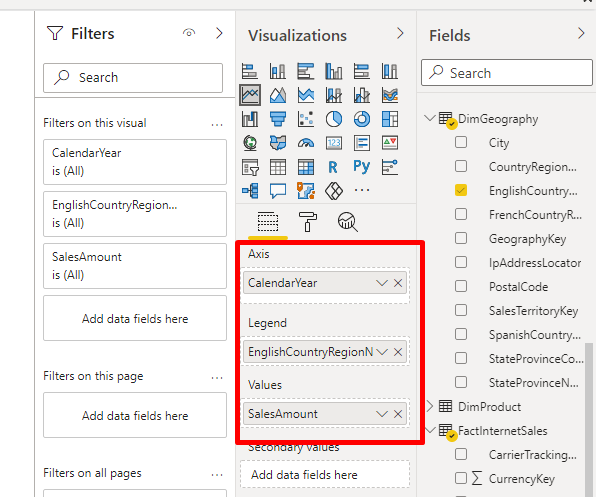
\includegraphics[width=13cm]{./img/img12.2.png}
            \end{center}
        \end{itemize}
        \item Puede definir los nombres de las hojas para indicar el tipo de reporte y la información. Establezca nombres descriptivos según la información que usted quiere facilitar.
        \begin{center}
            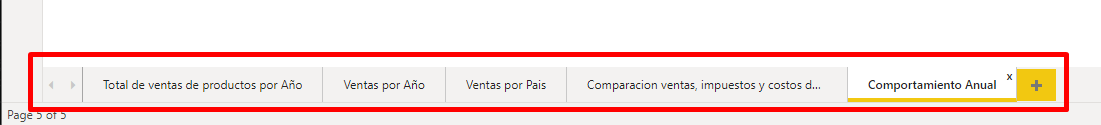
\includegraphics[width=13cm]{./img/img13.png}
        \end{center}
        \item Crearemos un reporte (gráfico de barras) con filtrado básico. 
        \begin{center}
            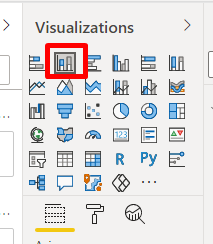
\includegraphics[width=6cm]{./img/img14.png}
        \end{center}
        \begin{itemize}
            \item Seleccionar Sales Amount, English Country Region Name y Order date/Calendar Year. Buscará la sección Basic Filtering y marcará Canada / United Kingdom.
            \begin{center}
                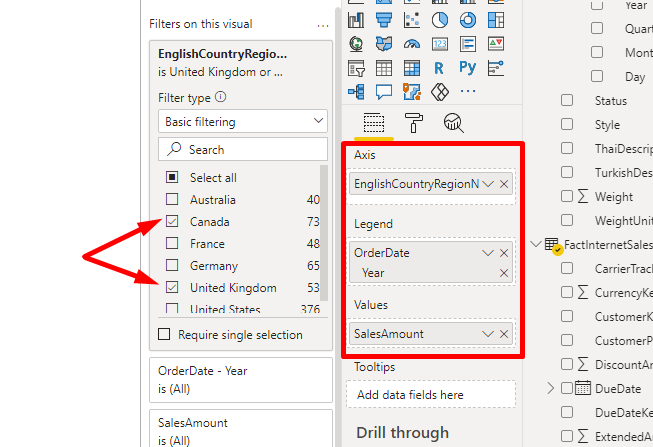
\includegraphics[width=8cm]{./img/img14.1.png}
            \end{center}
        \end{itemize}
        \item La siguiente gráfica es una Stacked Column Chart. 
        \begin{center}
            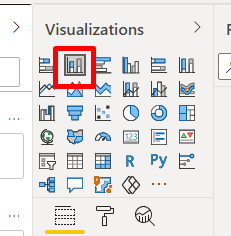
\includegraphics[width=5cm]{./img/img15.png}
        \end{center}
        \begin{itemize}
            \item Los atributos que utilizaremos son Sales Amount vs English ProductName vs Order Date/Calendar Year.
            \begin{center}
                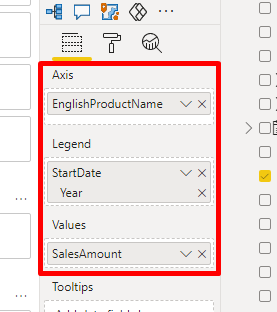
\includegraphics[width=5cm]{./img/img15.1.png}
            \end{center}
            \item Ahora incluya un filtro. Buscaremos productos que hayan vendido arriba de los \$400,000.
            \begin{center}
                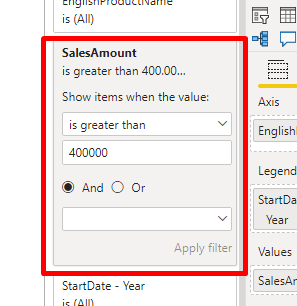
\includegraphics[width=5cm]{./img/img15.2.png}
            \end{center}
        \end{itemize}
        \item Incluya un Table con los siguientes campos: Sales Amount, English Product Name y Calendar Year.
        \begin{itemize}
            \item Seleccione Show as a Table.
            \begin{center}
                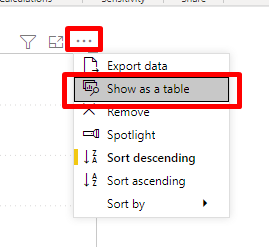
\includegraphics[width=5cm]{./img/img16.1.png}
            \end{center}
            \item Podrá visualizar el detalle de ventas.
            \begin{center}
                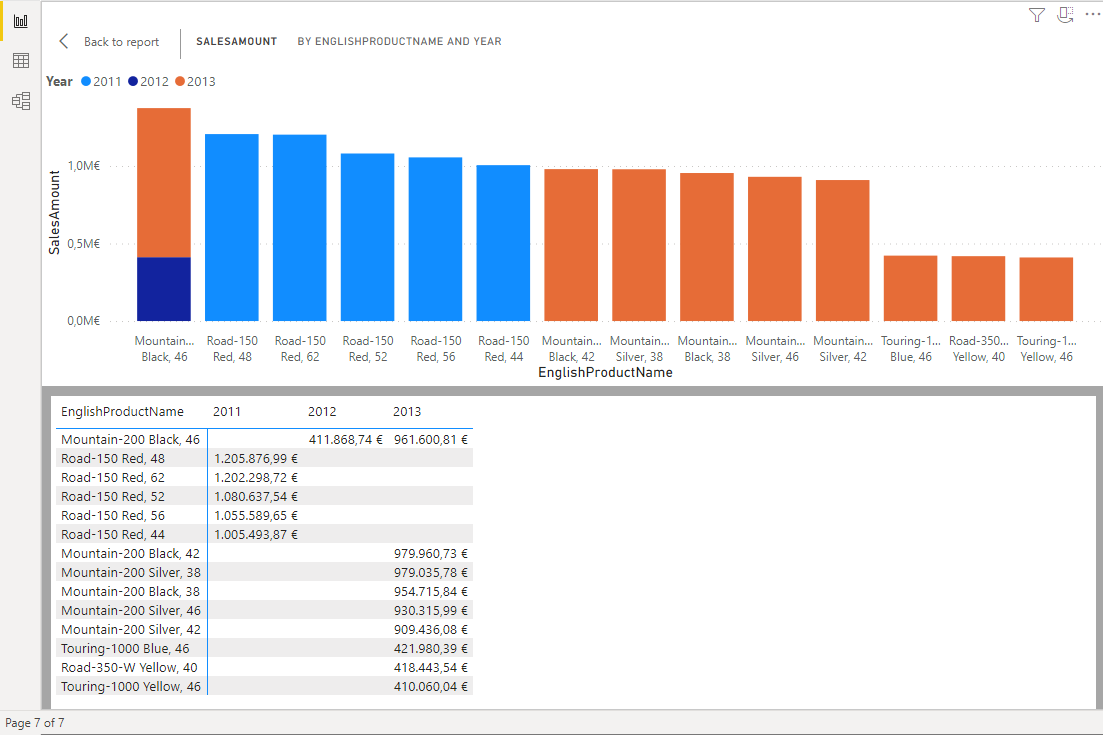
\includegraphics[width=13cm]{./img/img16.2.png}
            \end{center}
        \end{itemize}
        \item Cambie la orientación del reporte:
        \begin{center}
            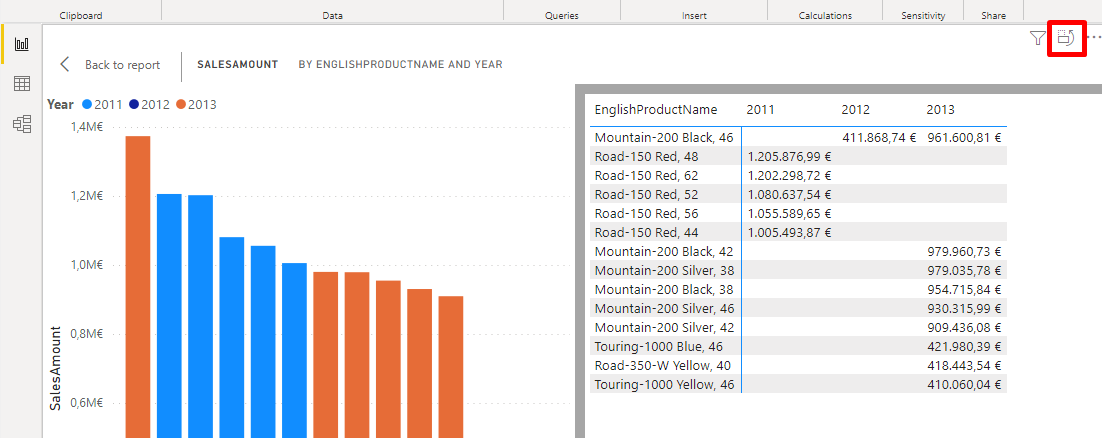
\includegraphics[width=13cm]{./img/img17.png}
        \end{center}
        \item Exporte su reporte para visualización.
    \end{enumerate}
    
    \newpage
    \section{Analisis de Resultados}
    Utilizando la base de datos Chinook, investigue cómo generar la dimensión de tiempo y luego, crear los siguientes reportes (tome en cuenta que se necesita conocer los valores en dinero):\\[0.1in]
    Se requiere saber cuáles son los artistas que más han vendido en la plataforma
    \begin{enumerate}[\tab 1.]
        \item Ventas por país contra año.\\[0.1in]
        Para este reporte se usaron dos visualizaciones, \textbf{Slicer} y \textbf{Column Chart}, para la primera visualización \textbf{(Slicer)} que se usa para filtrar por año se agregó el campo \textit{\textbf{InoviceDate}} de la tabla \textit{\textbf{Invoice}} y se seleccionó el subcampo \textit{\textbf{Year}}, posterior a eso se cambió el diseño la visualización para que no se vea como una lista simple si no para que se vea como botones; en el caso de la segunda visualización \textbf{(Column Chart)} se agregó el campo \textit{\textbf{BillingCountry}} de la tabla \textit{\textbf{Invoice}} en los \textit{Ejes} y el campo \textit{\textbf{Quantity}} de la tabla \textit{\textbf{InvoiceLine}} en los \textit{Valores}, posterior a eso se obtiene los resultados que se puede ver en la imagen donde se puede filtrar por año.
        \begin{center}
            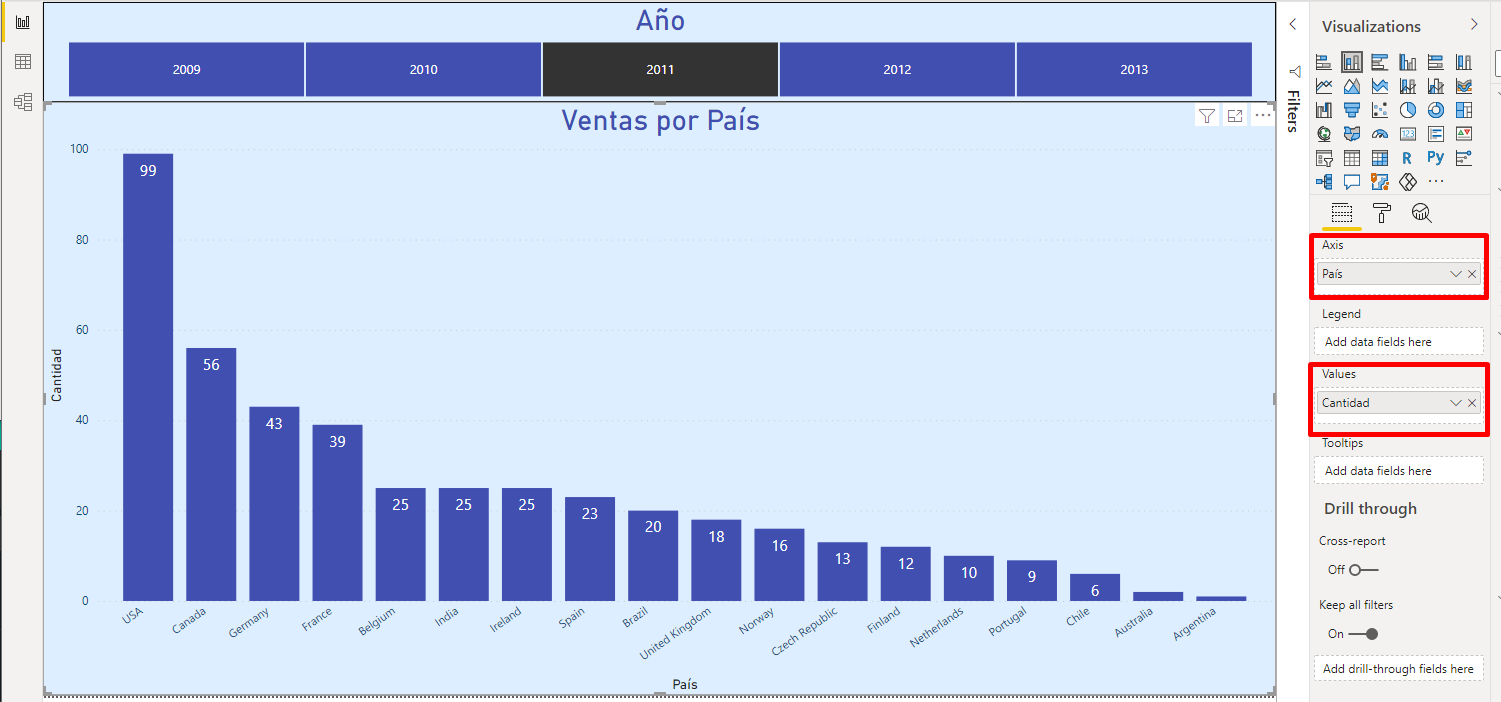
\includegraphics[width=13cm]{./img/img20.png}
        \end{center}
        \item Ventas por país (mapa).\\[0.1in]
        Para este reporte se usó solo una visualización, \textbf{Map}, en este caso se agregó el campo \textit{\textbf{BillingCountry}} de la tabla \textit{\textbf{Invoice}} en la \textit{Locación} y el campo \textit{\textbf{Quantity}} de la tabla \textit{\textbf{InvoiceLine}} en el \textit{Tamaño}, posterior a eso se obtiene los resultados que se puede ver en la imagen donde se ve que un círculo que su tamaño depende de la cantidad de ventas que se tenga en cada país.
        \begin{center}
            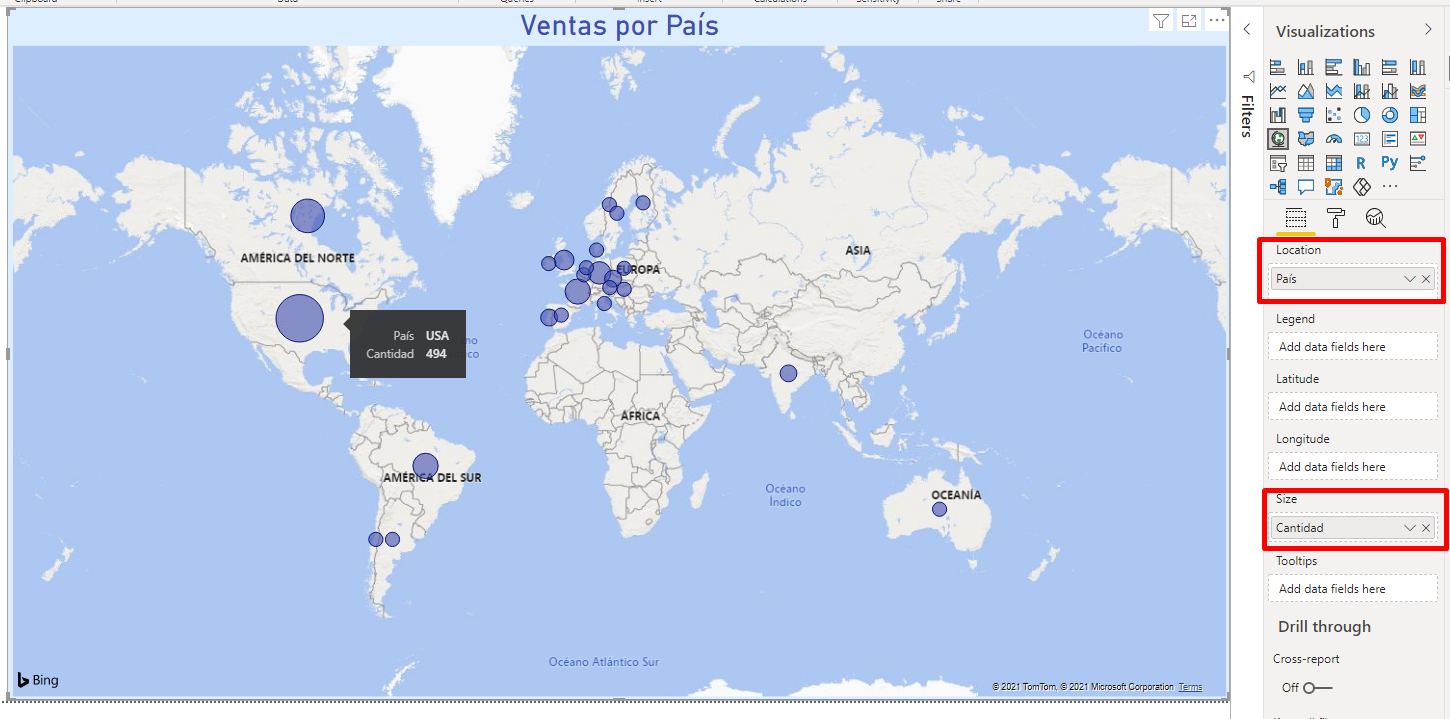
\includegraphics[width=13cm]{./img/img21.png}
        \end{center}
        \item Ventas realizadas por artista y año.\\[0.1in]
        Para este reporte se usaron dos visualizaciones, \textbf{Slicer} y \textbf{Column Chart}, para la primera visualización \textbf{(Slicer)} que se usa para filtrar por año se agregó el campo \textit{\textbf{InoviceDate}} de la tabla \textit{\textbf{Invoice}} y se seleccionó el subcampo \textit{\textbf{Year}}, posterior a eso se cambió el diseño la visualización para que no se vea como una lista simple si no para que se vea como botones; en el caso de la segunda visualización \textbf{(Column Chart)} se agregó el campo \textit{\textbf{Name}} de la tabla \textit{\textbf{Artist}} en los \textit{Ejes} y el campo \textit{\textbf{Quantity}} de la tabla \textit{\textbf{InvoiceLine}} en los \textit{Valores}, posterior a eso se obtiene los resultados que se puede ver en la imagen donde se puede filtrar por año.
        \begin{center}
            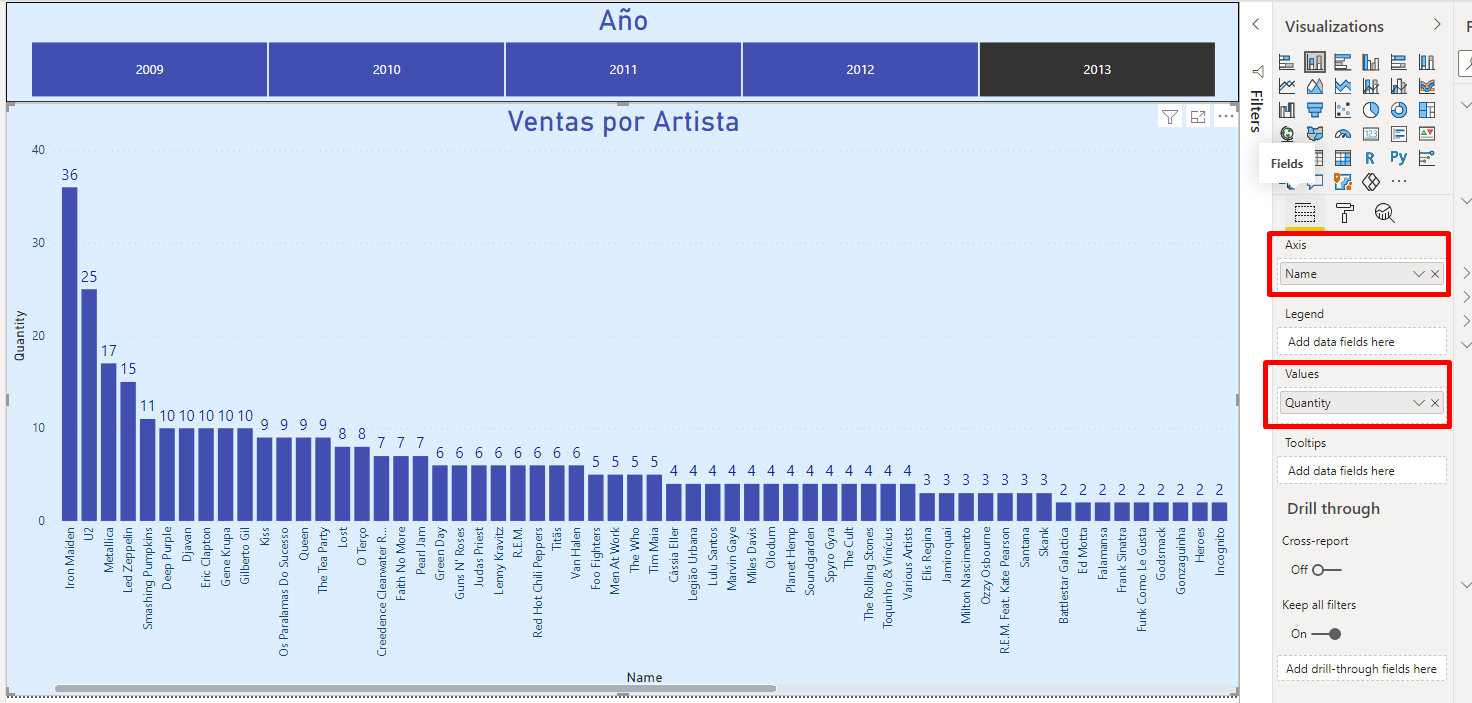
\includegraphics[width=13cm]{./img/img22.png}
        \end{center}
        \item Genere 4 reportes adicionales utilizando los datos que usted considere relevantes.\\[0.1in]
        \begin{itemize}
            \item Ventas por País divididas por 3 Géneros mas populares.\\[0.1in]
            Para este reporte se usó solo una visualización, \textbf{Map}, en este caso se agregó el campo \textit{\textbf{BillingCountry}} de la tabla \textit{\textbf{Invoice}} en la \textit{locación}, el campo \textit{\textbf{Quantity}} de la tabla \textit{\textbf{InvoiceLine}} en el \textit{tamaño} y el campo \textit{\textbf{Name}} de la tabla \textit{\textbf{Genre}} en la sección \textit{Leyenda}, posterior a eso se obtiene los resultados que se puede ver en la imagen donde se ve que un círculo que su tamaño depende de la cantidad de ventas que se tenga en cada país, pero a su ves este círculo está dividido en 3 que representa los 3 géneros más populares en el mundo.
            \begin{center}
                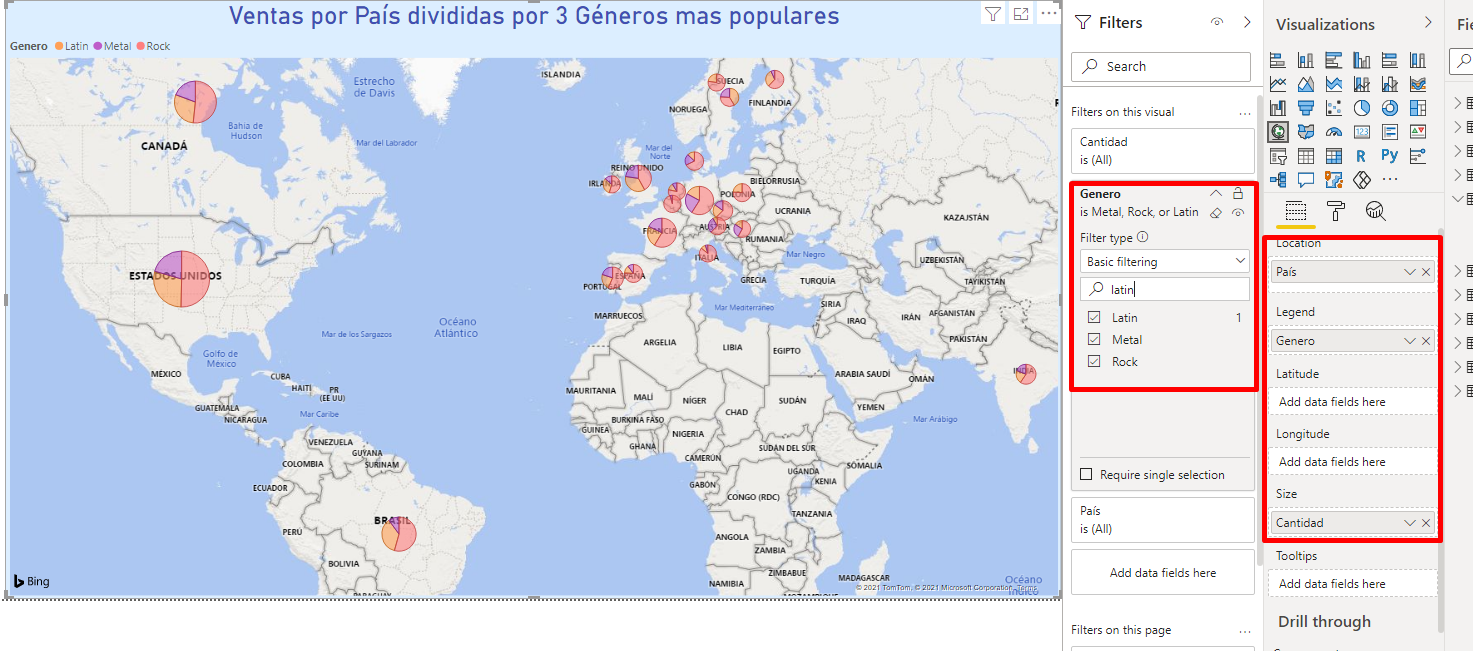
\includegraphics[width=13cm]{./img/img23.1.png}
            \end{center}
            \item Cantidad de Albumes por Artista.\\[0.1in]
            Para este reporte se usó solo una visualización, \textbf{Map}, en este caso se agregó el campo \textit{\textbf{Name}} de la tabla \textit{\textbf{Artist}} en los \textit{Ejes} y el campo \textit{\textbf{Title}} de la tabla \textit{\textbf{Album}} en los \textit{Valores}, posterior a eso se obtiene los resultados de los artistas que produjeron más álbumes.
            \begin{center}
                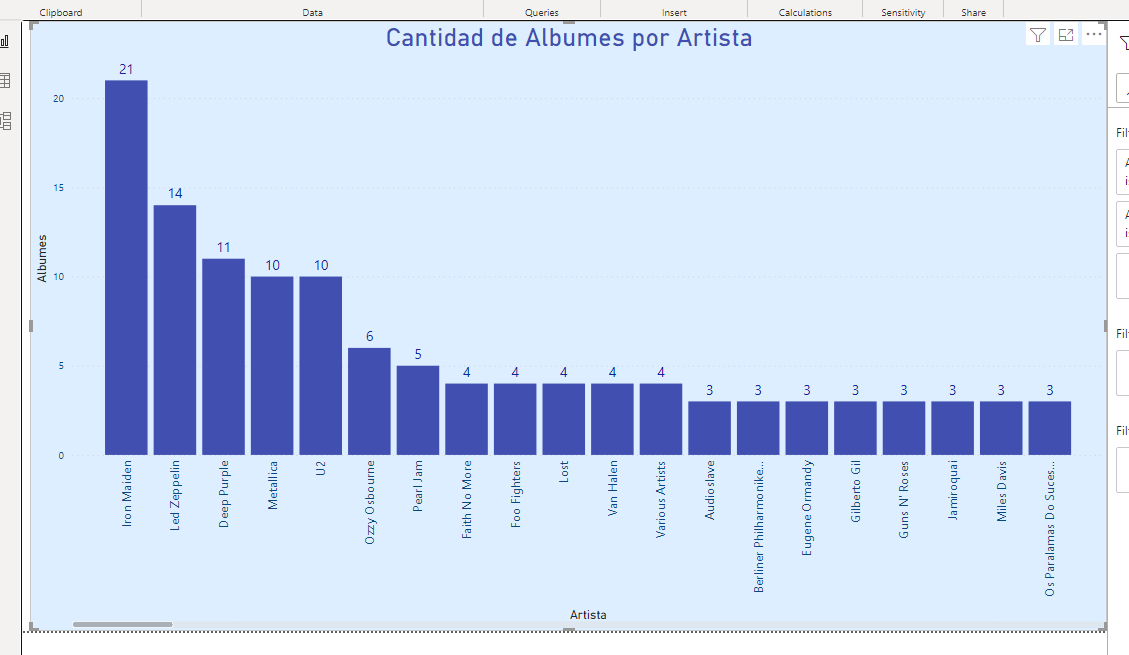
\includegraphics[width=13cm]{./img/img23.2.png}
            \end{center}
            \item Monto recaudado y cantidad vendidad por cada Album, filtrada por año.\\[0.1in]
            Para este reporte se usaron dos visualizaciones, \textbf{Slicer} y \textbf{Clustered Column Chart}, para la primera visualización \textbf{(Slicer)} que se usa para filtrar por año se agregó el campo \textit{\textbf{InoviceDate}} de la tabla \textit{\textbf{Invoice}} y se seleccionó el subcampo \textit{\textbf{Year}}, posterior a eso se cambió el diseño la visualización para que no se vea como una lista simple si no para que se vea como botones; en el caso de la segunda visualización \textbf{(Clustered Column Chart)} se agregó el campo \textit{\textbf{Title}} de la tabla \textit{\textbf{Album}} en los \textit{Ejes} y los campos \textit{\textbf{UnitPrice}} y \textit{\textbf{Quantity}} de la tabla \textit{\textbf{InvoiceLine}} en los \textit{Valores}, posterior a eso se obtiene los resultados donde se puede observar la cantidad vendida respecto al monto recaudado y todo eso filtrado por años.
            \begin{center}
                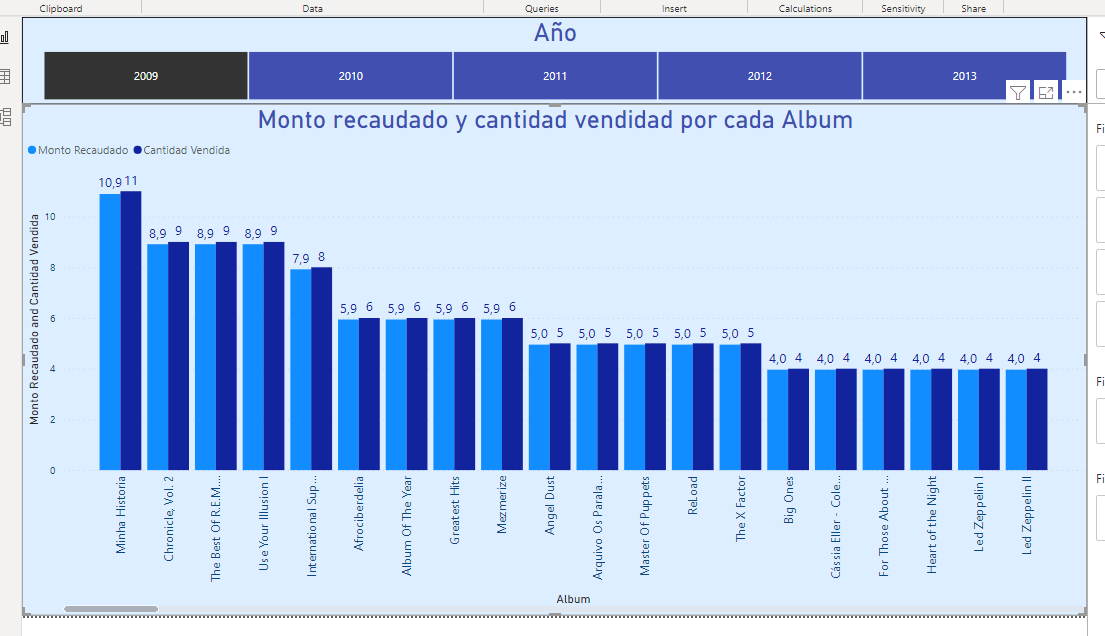
\includegraphics[width=13cm]{./img/img23.3.png}
            \end{center}
            \item Cantidad de ventas por vendedores, filtrada por año.\\[0.1in]
            Para este reporte se usaron dos visualizaciones, \textbf{Slicer} y \textbf{Column Chart}, para la primera visualización \textbf{(Slicer)} que se usa para filtrar por año se agregó el campo \textit{\textbf{InoviceDate}} de la tabla \textit{\textbf{Invoice}} y se seleccionó el subcampo \textit{\textbf{Year}}, posterior a eso se cambió el diseño la visualización para que no se vea como una lista simple si no para que se vea como botones; en el caso de la segunda visualización \textbf{(Column Chart)} se agregó el campo \textit{\textbf{CompleteName}} de la tabla \textit{\textbf{Employee}} en los \textit{Ejes} y el campo \textit{\textbf{CustomerId}} de la tabla \textit{\textbf{Invoice}} en los \textit{Valores}, posterior a eso se obtiene los resultados donde se puede observar la cantidad de ventas respecto al vendedor y todo eso filtrado por años.
            \begin{center}
                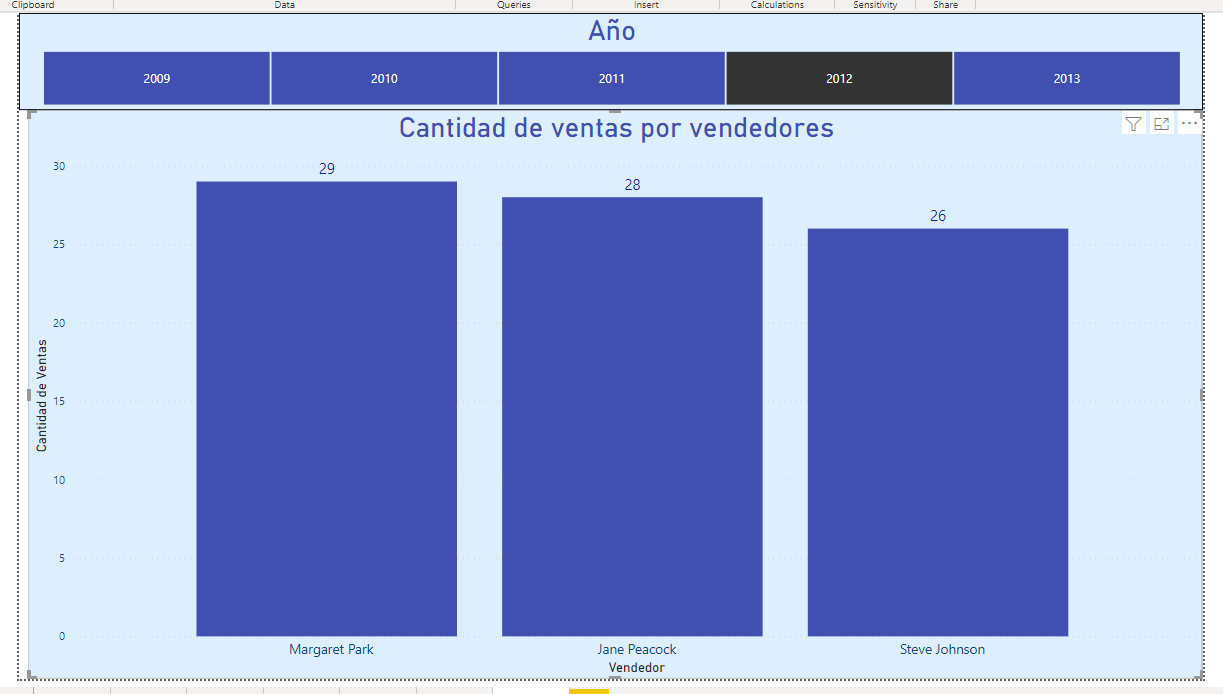
\includegraphics[width=13cm]{./img/img24.4.png}
            \end{center}
        \end{itemize}
        \item Investigue cómo visualizar los reportes que ha creado en dispositivos móviles.\\[0.1in]
        \begin{itemize}
            \item Primero nos dirigimos a la sección \textbf{View} y seleccionamos la opción \textbf{Mobile layout}.
            \begin{center}
                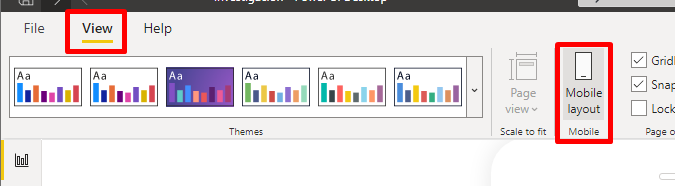
\includegraphics[width=6cm]{./img/img25.1.png}
            \end{center}
            \item Al lado derecho veremos todas las visualizaciones que tenemos en las diferentes páginas.
            \begin{center}
                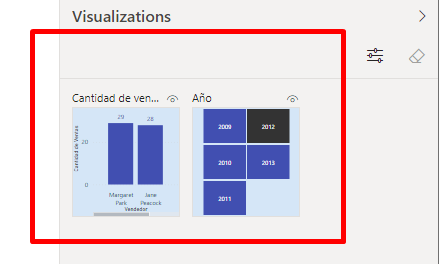
\includegraphics[width=6cm]{./img/img25.2.png}
            \end{center}
            \item Solo basta con arrastrarlas al teléfono y acomodarlas como se crea conveniente.
            \begin{center}
                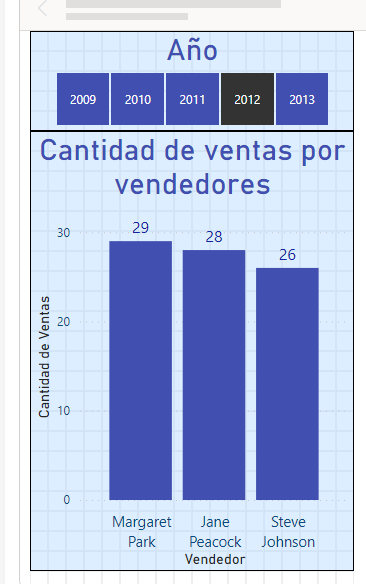
\includegraphics[width=6cm]{./img/img25.3.png}
            \end{center}
            \item Una vez terminado nos dirigimos a la sección \textbf{Home} y hacemos clic en el botón \textbf{Publish}.
            \begin{center}
                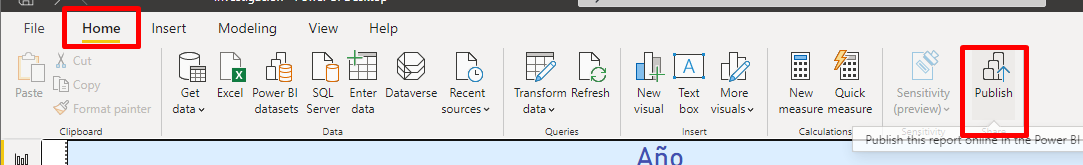
\includegraphics[width=13cm]{./img/img25.4.png}
            \end{center}
            \item En la ventana que se muestra seleccionamos \textbf{'My workspace'} y hacemos clic en el botón \textbf{Select}.
            \item Esperamos a que el reporte se suba a la nube.
            \item Ahora desde el teléfono ingresamos a la aplicación móvil de \textbf{Power BI} con la misma cuenta que iniciamos sesión en la aplicación de escritorio.
            \item En la sección de \textbf{Accesos rápidos} buscamos el DashBoard que guardamos anteriormente e ingresamos a este.
            \item Nos cargara los reportes con el diseño que se le puso en los pasos anteriores.
        \end{itemize}
    \end{enumerate}
    
    \newpage
    \section{CONCLUSIONES}
    \begin{itemize}
        \item Se logro crear diferentes reportes desde una misma base de datos sin tanta dificultad como seria hacerlo con consultas SQL.
        \item Se logro exportar de manera satisfactoria nuestros reportes en un archivo sin error alguno.
        \item Es muy sencillo tener todos los reportes creados en la palma de nuestra mano, como ya se vio es muy sencillo poder visualizar los reportes desde nuestro teléfono móvil ya sea su Sistema Operativo Android o IOS.
    \end{itemize}
    
    \newpage
    \section{WEBGRAFIA}
    \begin{itemize}
        \item GitHub. (2015). ExploraVisualizaconR.\\
        Recuperado de \textcolor{azul}{\url{https://github.com/fcharte/ExploraVisualizaconR}}
        \item Code Like a Girl. (2018). Análisis y visualización de datos con Pandas \& MatPlotLib.\\
        Recuperado de \textcolor{azul}{\url{https://code.likeagirl.io/analisis-y-visualizacion-de-datos-con-pandas-matplotlib-85ee4d7b4cad}}
        \item Analitics Lane. (2018). Visualización de datos en Python con Seaborn.\\
        Recuperado de \textcolor{azul}{\url{https://www.analyticslane.com/2018/07/20/visualizacion-de-datos-con-seaborn/}}
        \item Microdsosft Docs. (2020). Tutorial de Python: Explorar y visualizar datos.\\
        Recuperado de \textcolor{azul}{\url{https://docs.microsoft.com/es-es/sql/machine-learning/tutorials/python-taxi-classification-explore-data?view=sql-server-2017}}
        \item Hernández, A y Chacón, H. (2019). Manipulación, análisis y visualización de datos de la encuesta demográfica y de salud familiar con el programa R.\\
        Recuperado de \textcolor{azul}{\url{http://www.scielo.org.pe/scielo.php?script=sci_arttext&pid=S1726-46342019000100019&lng=es&nrm=iso&tlng=es}}
        \item GitHub. (2019). Analisis-Endes-Peru.\\
        Recuperado de \textcolor{azul}{\url{https://github.com/horaciochacon/Analisis-Endes-Peru}}
    \end{itemize}
\end{document}